\documentclass[12pt]{article}

\usepackage[utf8]{inputenc}
\usepackage[T1]{fontenc}
\usepackage{geometry}
\usepackage{amssymb}
\usepackage{amsmath}
\geometry{a4paper}
\usepackage{graphicx}

\begin{document}

The coil is assumed to be centered at origin and axis along $z$-axis (hence cylindrical symmetry about $z$-axis) as shown in the figure below:

\begin{center}
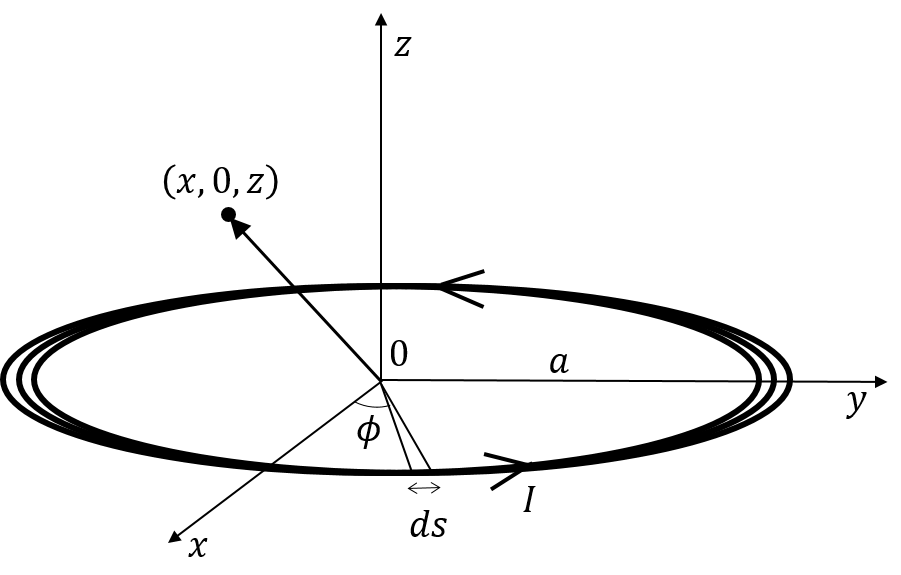
\includegraphics[width=100mm]{coil.png}
\end{center}

Magnetic vector potential is given by:
$$ \vec{A}=\frac{\mu_0I}{4\pi}\int \frac{d\vec{s}}{R} $$
where $Id\vec{s}$ is the current multiplied by the line element on the coil, $R$ is the distance between current element and the point where $\vec{A}$ is to be calculated. Co-ordinates of the current element, as shown in the figure, are $(a\cos\phi,a\sin\phi,0)$. Due to cylindrical symmetry, calculation made in $x$-$z$ plane can be generalized for any position later, so first $\vec{A}$ is calculated at $\left(x,0,z\right)$, hence:
$$ R=\sqrt{(x-a\cos\phi)^2+a^2\sin^2\phi+z^2}=\sqrt{x^2+a^2+z^2-2ax\cos\phi} $$
and since $Id\vec{s}=-aI\sin\phi\,d\phi\,\hat{i}+aI\cos\phi\,d\phi\,\hat{j}$, vector potential becomes:
$$ \vec{A}=\frac{\mu_0I}{4\pi}\left[\int_{0}^{2\pi} \frac{-a\sin\phi\,d\phi\,\hat{i}}{\sqrt{x^2+a^2+z^2-2ax\cos\phi}}+\int_{0}^{2\pi} \frac{a\cos\phi\,d\phi\,\hat{j}}{\sqrt{x^2+a^2+z^2-2ax\cos\phi}}\right] $$
Since $\sin$ is odd and $\cos$ is even, first term vanishes. The direction $\hat{j}$ in second term should be changed to $\hat\phi$, so that later we can generalize $\vec{A}$ to any point $(x,y,z)$ (note that $\hat{j}$ and $\hat\phi$ are same on $x$-$z$ plane). Now, $\vec{A}$ can be written as:
\begin{align}\vec{A} &= \frac{\mu_0Ia}{2\pi}\int_0^\pi \frac{\cos\phi\,d\phi}{\sqrt{x^2+a^2+z^2-2ax\cos\phi}}\hat\phi \nonumber \\
&= \frac{\mu_0Ia}{2\pi}\int_0^\pi \frac{\cos\phi\,d\phi}{\sqrt{(x+a)^2+z^2-2ax(1+\cos\phi)}}\hat\phi \nonumber \\
&= \frac{\mu_0Ia}{2\pi}\int_0^\pi \frac{\cos\phi\,d\phi}{\sqrt{(x+a)^2+z^2-4ax\cos^2(\phi/2)}}\hat\phi \nonumber \end{align}
Define $k=\sqrt{\frac{4ax}{(x+a)^2+z^2}}$ and $\phi=\pi-2\alpha$, so that:
$$ \vec{A}=\frac{\mu_0Ia}{2\pi}\int_0^{\pi/2} \frac{k\left(-\cos2\alpha\right)\,d\alpha}{\sqrt{ax}\sqrt{1-k^2\sin^2\alpha}}\hat\phi = \frac{\mu_0Ik}{2\pi}\sqrt{\frac{a}{x}}\int_0^{\pi/2} \frac{\left(2\sin^2\alpha-1\right)\,d\alpha}{\sqrt{1-k^2\sin^2\alpha}}\hat\phi $$
From the definitions of the Elliptic Integrals of first and second kind:
$$ K\left(k\right)=\int_0^{\pi/2}\frac{d\alpha}{\sqrt{1-k^2\sin^2\alpha}} $$
$$ E\left(k\right)=\int_0^{\pi/2}\sqrt{1-k^2\sin^2\alpha}\,d\alpha $$
respectively, the vector potential can be written as:
$$ \vec{A}=\frac{\mu_0I}{2\pi}\sqrt{\frac{a}{x}}\left[K(k)\left( \frac{2}{k}-k \right) -\frac{2}{k}E(k) \right]\hat\phi $$
From this, magnetic field can be calculated. Curl in cylindrical co-ordinates is given as:
$$ \nabla\times\vec{A}=\left(\frac{1}{r}\frac{\partial A_z}{\partial\phi}-\frac{\partial A_\phi}{\partial z}\right)\hat{r}+\left(\frac{\partial A_r}{\partial z}-\frac{\partial A_z}{\partial r}\right)\hat{\phi}+\frac{1}{r}\left(\frac{\partial(rA_\phi)}{\partial r}-\frac{\partial A_r}{\partial\phi}\right)\hat{z} $$
Since the point at which the magnetic field is calculated lies in $x$-$z$ plane, $x$ is equivalent to $r$ in the expression of $\vec{A}$. Derivatives of $k$ are:
$$ \frac{\partial k}{\partial z}=\frac{-z\left(4ax\right)^{3/2}}{\left(\left(x+a\right)^2+z^2\right)^{3/2}\left(4ax\right)}=-\frac{k^3z}{4ax} $$
$$ \frac{\partial k}{\partial x}=\frac{-\sqrt{4ax}\left(x+a\right)\left(4ax\right)}{\left(\left(x+a\right)^2+z^2\right)^{3/2}\left(4ax\right)}+\frac{\sqrt{a}}{\left(\left(x+a\right)^2+z^2\right)^{1/2}\sqrt{x}}=-\frac{k^3\left(x+a\right)}{4ax}+\frac{k}{2x} $$
Derivatives of Elliptic Integrals are:
$$ \frac{\partial K}{\partial k}=\frac{E}{k\left(1-k^2\right)}-\frac{K}{k} $$
$$ \frac{\partial E}{\partial k}=\frac{E-K}{k} $$
From these:
\begin{align}\frac{\partial A_\phi}{\partial z}&=-\frac{\mu_0I}{2\pi}\sqrt{\frac{a}{x}}\frac{k^3z}{4ax}\left[\frac{\partial K}{\partial k}\left(\frac{2}{k}-k\right)-K\left(1+\frac{2}{k^2}\right)+\frac{2E}{k^2}-\frac{2}{k}\frac{\partial E}{\partial k}\right] \nonumber \\ &=\frac{\mu_0Ikz}{4\pi}\sqrt{\frac{1}{ax^3}}\left[K-\frac{E(2-k^2)}{2(1-k^2)}\right] \nonumber \end{align}
\begin{align}\frac{\partial(xA_\phi)}{\partial x}&=\frac{\mu_0I\sqrt{a}}{2\pi}\Bigg[\frac{1}{2\sqrt{x}}\left(K\left(\frac{2}{k}-k\right)-\frac{2E}{k}\right) \nonumber \\ & +\sqrt{x}\left(\frac{\partial K}{\partial k}\left(\frac{2}{k}-k\right)-K\left(1+\frac{2}{k^2}\right)+\frac{2E}{k^2}-\frac{2}{k}\frac{\partial E}{\partial k}\right)\left(\frac{-k^3(x+a)}{4ax}+\frac{k}{2x}\right)\Bigg] \nonumber \\
&=\frac{\mu_0Ik}{4\pi}\sqrt{\frac{x}{a}}\left(K+\frac{k^2(x+a)-2x}{2x(1-k^2)}E\right) \nonumber \end{align}
So the magnetic field is:
\begin{align} \vec{B}&=-\frac{\partial A_\phi}{\partial z}\hat{r}+\frac{1}{r}\frac{\partial(rA_\phi)}{\partial r}\hat{z} \nonumber \\
& =\frac{\mu_0Ik}{4\pi}\sqrt{\frac{1}{ax^3}}\left[-\left( K-\frac{E(2-k^2)}{2(1-k^2)}\right)z\hat{r}+x\left(K+\frac{k^2(x+a)-2x}{2x(1-k^2)}E\right)\hat{z}\right] \nonumber \end{align}
By cylindrical symmetry, this expression can be readily generalized for any $(x,y,z)$. Let $r=\sqrt{x^2+y^2}$, so:
$$ \vec{B}=\frac{\mu_0Ik}{4\pi}\sqrt{\frac{1}{ar^3}}\left[-\left( K-\frac{E(2-k^2)}{2(1-k^2)}\right)z\hat{r}+r\left(K+\frac{k^2(r+a)-2r}{2r(1-k^2)}E\right)\hat{z}\right] $$
where:
$$ k=\sqrt{\frac{4ar}{(r+a)^2+z^2}} $$
$$ K=\int_0^{\pi/2}\frac{d\alpha}{\sqrt{1-k^2\sin^2\alpha}} $$
$$ E=\int_0^{\pi/2}\sqrt{1-k^2\sin^2\alpha}\,d\alpha $$
Before coding, please verify the definition of elliptic integrals in the language you are coding. Mathematica and MATLAB have different definitions for elliptic integrals than mentioned above. \\

To calculate magnetic field for the coil axis in arbitrary direction, e.g. $\left(a_x,a_y,a_z\right)$, $z$-axis needs to be rotated in the direction $\left(\sin\theta\cos\phi,\sin\theta\sin\phi,\cos\theta\right)$, which is basically rotation in $x$-$z$ plane by $\theta$ (about $y$-axis) followed by rotation in $x$-$y$ plane by $\phi$ (about $z$-axis), where $\theta=\cos^{-1}\left(a_z/\sqrt{a_x^2+a_y^2+a_z^2}\right)$ and $\phi=\tan^{-1}\left(a_y/a_x\right)$. For $\phi$, the correct quadrant needs to be considered, which is taken care by atan2() function in FORTRAN. The corresponding rotation matrix is thus:

$$
R_{\theta\phi}=
\begin{bmatrix}
\cos\phi & -\sin\phi & 0 \\
\sin\phi & \cos\phi & 0 \\
0 & 0 & 1 \\
\end{bmatrix}
\cdot
\begin{bmatrix}
\cos\theta & 0 & \sin\theta \\
0 & 1 & 0 \\
-\sin\theta & 0 & \cos\theta \\
\end{bmatrix}
=
\begin{bmatrix}
\cos\theta\cos\phi & -\sin\phi & \sin\theta\cos\phi \\
\cos\theta\sin\phi & \cos\phi & \sin\theta\sin\phi \\
-\sin\theta & 0 & \cos\theta \\
\end{bmatrix}
$$

If magnetic field $\vec{B}$ is required at a given point $\vec{x}=\left(x,y,z\right)$, then first $\vec{x}$ needs to be rotated to $\vec{x}'=R_{\theta\phi}^{-1}\cdot\vec{x}$ and magnetic field should be calculated at $\vec{x}'$, say it is $\vec{B}'$, which then should be rotated back to get the required magnetic field, i.e., $\vec{B}=R_{\theta\phi}\cdot\vec{B}'$. The inverse rotation of position can be simply written as:

\[
\begin{bmatrix}
x' \\
y' \\
z' \\
\end{bmatrix}
=
\begin{bmatrix}
\cos\theta\cos\phi & \cos\theta\sin\phi & -\sin\theta \\
-\sin\phi & \cos\phi & 0 \\
\sin\theta\cos\phi & \sin\theta\sin\phi & \cos\theta \\
\end{bmatrix}
\cdot
\begin{bmatrix}
x \\
y \\
z \\
\end{bmatrix}
=
\begin{bmatrix}
\left(x\cos\phi+y\sin\phi\right)\cos\theta-z\sin\theta \\
-x\sin\phi+y\cos\phi \\
\left(x\cos\phi+y\sin\phi\right)\sin\theta+z\cos\theta \\
\end{bmatrix}
\]

\end{document}
